\documentclass{ctexart}
\usepackage[utf8]{inputenc}
\usepackage{graphicx}
\usepackage{tikz}
\usetikzlibrary{shapes,arrows}


\title{图的模板类设计}
\author{陈科辉 Keiver Pabula}
\date{24 November,2022}
\begin{document}
\maketitle

\section{设计思路}
首先我先创建一个图,然后输入边,节点的个数和节点的源是哪一个。初始化值,让从起点0到各个节点的值为无穷大,而从起点0到终点0的值为0;进行最多n-1次的遍历操作,对所有的边都进行松弛,而松弛分两步走,判断从起点到a(dist(a))是否大于从起点到b(dist(b))+边ab的权重(weight),如果大于则将从起点到b(dist(b))+边ab的权重(weight)赋值给起点到a(dist(a));最后一部判断负边环遍历都结束后,若再进行一次遍历,还能得到s到某些节点更短的路径的话,则说明存在负环路。

\section{测试结果}
Bellman-Ford算法结果:
\begin{center}
  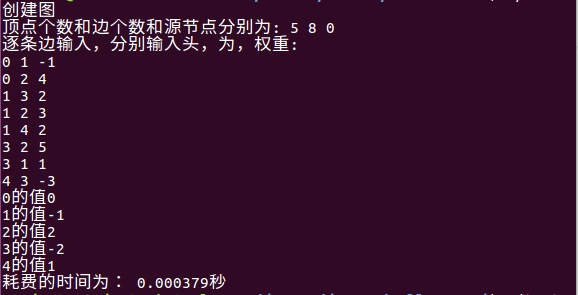
\includegraphics[scale=0.6]{ss1.png}
  \hspace{0.1in}
\end{center}
\begin{center}
  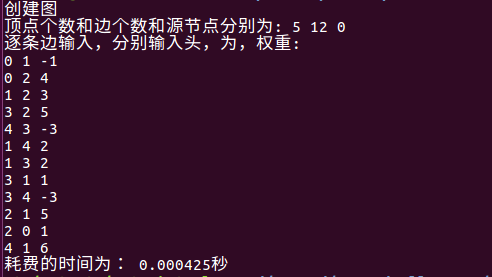
\includegraphics[scale=0.5]{ss2.png}
  \hspace{0.1in}
\end{center}
\begin{center}
  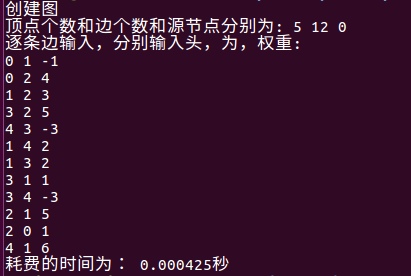
\includegraphics[scale=0.6]{ss3.png}
  \hspace{0.1in}
\end{center}
\begin{center}
  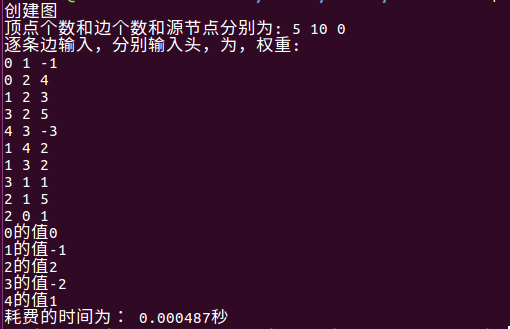
\includegraphics[scale=0.5]{ss4.png}
  \hspace{0.1in}
\end{center}
\begin{center}
  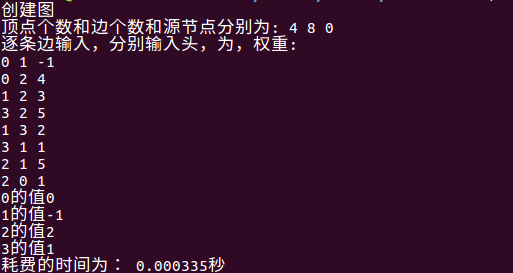
\includegraphics[scale=0.6]{ss5.png}
  \hspace{0.1in}
\end{center}
\begin{center}
  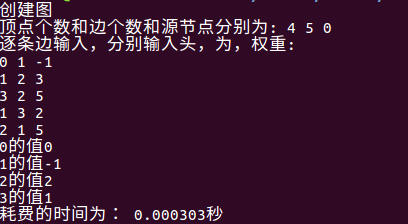
\includegraphics[scale=0.6]{ss7.png}
  \hspace{0.1in}
\end{center}
\begin{center}
  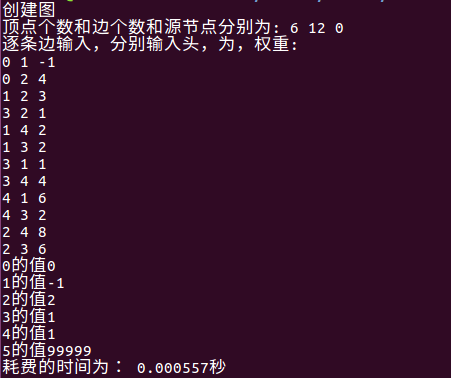
\includegraphics[scale=0.5]{ss8.png}
  \hspace{0.1in}
\end{center}
可以看到当顶点和边变多时,所消耗的时间就会越长,因此边或节点的个数与时间两者呈正比。


\end{document}
